\section{Development Architectural View}

Because we are using nxtOSEK as our operating system for the bus, we can program using either C or C++, see \ref{nxtOSEK} for more details. Because we can split the program cleanly into modular components as shown in the previous diagram \ref{fig:components}, we will program using the object-oriented programming paradigm with C++. 

Using the separated components as the baseline, we now create a class diagram that is less abstract than the component separation, which we will be used as the software architecture of the model (the programming logic of the bus) implementation. See Figure \ref{fig:softwareArchitecture}. %Using this diagram, we will later create precise interfaces for all its classes. The dark blue boxes signify the physical sensors that the program will need to communicate with. See figure \ref{fig:softwareArchitecture} 

\begin{figure}[ht]
    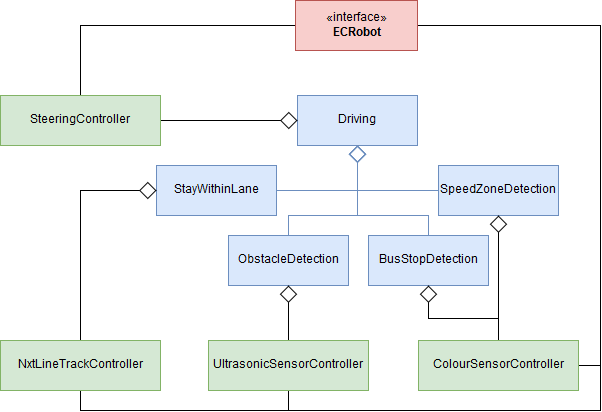
\includegraphics[width=\textwidth]{Images/Design/designClassDiagram.png}
    \caption{Class diagram over the software for the model of the bus}
    \label{fig:softwareArchitecture}
\end{figure}

%The arrows on the figure signify function calls, e.g. if an arrow points from object A to B, it means that object A will call functions from object B. To better describe the concerns of each class on the diagram, we've written an example of one function call that might occur between the objects on each edge. This part isn't intended to be extremely precise, however, it helps communicate how we are planning to use object-oriented programming for information hiding and abstraction. See the diagram in figure \ref{fig:softwareArchitecture}

The blue tinted classes are the same as were shown on the previous class diagram over the major components (Figure \ref{fig:components}). 

The green tinted classes are sensor controller classes, that will be coupled closely to the corresponding sensors of the bus. These classes are needed since sensors sometimes need to be calibrated and are also are known to produce unreliable results that need to be sorted out, as was established in prior sensor testing sections \ref{Analysis:ultrasonicTests} and \ref{CamAnalysis}. The point of these classes is to allow the logic of the rest of the program to disregard any hardware specifics, and simply trust the result that they receive. 

The 

This means:
The \code{SteeringController} contains both the back motor used to control the speed of the bus. The \code{ColourSensorController} is a shared resource used by both the \code{SpeedZoneDetection} and the \code{BusStopDetection}-components.



Something to note, which is not mentioned on the diagram, is that we have also planned to write a program separate from the system that normally steers the bus. This program has the job of allowing us to test the steering algorithms of the bus on a computer. The idea is that we can visually see where the algorithm would suggest the bus should drive all whilst seeing NXTCam sensor data displayed visually on screen. 

To ensure a stable connection, we will make the communication between the bus and the computer go through a USB cable rather than through Bluetooth signal, which the NXT Brick would also allow. This means that the final program will also contain a \code{UsbCommunicationController} class to handle this interaction. This is not visible on the above class diagram, since the class is only planned as a testing tool.